% DO NOT COMPILE THIS FILE DIRECTLY!
% This is included by the other .tex files.
\section{Вовед во околини за програмирање}

\begin{frame}{Програмирање (1)}
\begin{itemize}
\item Програмите, што компјутерот ги извршува се последователност од нули и
единици, затоа што тоа е единствениот јазик кој што компјутерот го разбира
\item Програмерите ги пишуваат своите програми на јазици за програмирање, кои
што се разбирливи за нив 
\item Програма напишана во јазик за програмирање ја нарекуваме \textbf{изворна програма}
\end{itemize}
\end{frame}

\begin{frame}{Програмирање (2)}
\begin{itemize}
  \item За пишување програми често се користат \textbf{околини за развој}
  \item Програмата се внесува преку текстуален уредувач
  \item Потоа се врши преведување на програмата (компајлирање)
  \item Со тоа се создава извршна програма т.е. програма
напишана во јазикот на компјутерот
\end{itemize}
\end{frame}

\begin{frame}{Елементи на околините за развој}
Околината за развој е составена од повеќе програми, кои го олеснуваат
целокупниот развој на една програма
\begin{itemize}
  \item текст уредувач (text editor)
  \item преведувач (компајлер - compiler)
  \item дебагер (debugger)
  \item интеграција на библиотеки со функции
  \item поврзувач (linker)
\end{itemize}
\end{frame}

\begin{frame}{Текст уредувач (text editor)}
\begin{itemize}
  \item Програма која овозможува внесување и уредување на текстот на изворната
  програма
  \item Овозможува зачувување на програми и вчитување на веќе напишани програми
  за нивно повторно уредување 
  \item Означување на клучните зборови и команди во изворната програма (syntax
  highlighting)
\end{itemize}
\end{frame}

\begin{frame}{Текст уредувач (text editor)}
\begin{itemize}
  \item Ја преобразува (преведува) изворната програма од јазикот за програмирање во кој е напишана во јазик разбирлив за компјутерот
  \item Се разликуваат два вида преведувачи: \textbf{интерпретери} и \textbf{компајлери} 
  \item Интерпретер е преведувач кој ја \emph{обработува одделно секоја команда}, ја
  проверува за грешки и ја извршува, по што поминува на следната команда  итн.
  \item Компајлер е преведувач кој ја \emph{обработува целата програма}, ја проверува
  за грешки и ја преведува, по што се добива извршната програма.
  \begin{itemize}
  \item Така добиената извршна програма може да се извршува
  \end{itemize}
\end{itemize}
\end{frame}

% Define block styles
\tikzstyle{block} = [rectangle, draw, fill=blue!20,
text width=5em, text centered, rounded corners, minimum height=4em]
\tikzstyle{line} = [draw, -latex']

\begin{frame}[fragile,shrink=20]{Тек на преведување и извршување на програма}
Фаза 1 - преведување на програмата
\begin{center}
\begin{tikzpicture}[node distance = 3cm, auto]
    % Place nodes
    \node [block] (compiler) {Преведувач\\(компајлер)};
    \node [block, below of=compiler, node distance=2cm] (source) {Изворна
    програма}; 
    \node [block, right of=compiler] (computer) {Компјутер};
    \node [block, right of=computer] (executable) {Програма во меморија};
    % Draw edges
    \path [line] (compiler) -> node {} (computer);
    \path [line] (source) -| node {} (computer);
    \path [line] (computer) -> node {} (executable);
\end{tikzpicture}
\end{center}
Фаза 2 - извршување на програмата
\begin{center}
\begin{tikzpicture}[node distance = 3cm, auto]
    % Place nodes
    \node [block] (programm) {Програма во меморија};
    \node [block, below of=programm] (data) {Влезни податоци};
    \node [block, right of=programm] (computer) {Компјутер};
    \node [block, text width=3cm, right of=computer] (executable) {Резултат од
    извршувањето на програмата};
    % Draw edges
    \path [line] (programm) -> node {} (computer);
    \path [line] (data) -| node {} (computer);
    \path [line] (computer) -> node {} (executable);
\end{tikzpicture}
\end{center}
\end{frame}

\begin{frame}{Дебагер (debugger)}
\begin{itemize}
  \item Компајлерите и интерпретерите ги откриваат грешките (синтаксички) во
  програмата поради не правилно користење на јазикот за програмирање
  \item Друг вид на грешки се логичките грешки
  \begin{itemize}
  \item Програмата не го прави тоа за кое што е наменета 
  \item Се откриваат многу тешко
  \end{itemize}
  \item Дебагер е програма која помага при барање на логичките грешки
  \begin{itemize}
  \item Овозможува следење на извршувањето на програмата чекор по чекор
  \end{itemize}
\end{itemize}
\end{frame}

\begin{frame}{Интеграција на библиотеки со функции}
\begin{itemize}
  \item Интегрирање и користење на претходно создадени и проверени модули (потпрограми), уште наречени и функции
  \item Ваквиот начин на организација на програмите има голем број на предности
  \item Повторно искористување на готови функционалности
  \item Пример библиотеки
  \begin{itemize}
    \item За управување со стандардниот влез и излез
    \item За стандардни математички операции 
  \end{itemize}
\end{itemize}
\end{frame}

\begin{frame}{Поврзувач (linker)}
\begin{itemize}
  \item Понекогаш програмата е премногу голема за да се напише во една датотека
  \begin{itemize}
    \item различните делови може да се пишуваат од различни програмери.
    \item некои делови од дадена програма можат да бидат искористени и во друга програма 
    \item Одделно компајлираните делови е неопходно да бидат обединети во една
    цела извршна програма со помош на \textbf{поврзувачот}
    \item Друга улога на поврзувачот е да ги „сврзе“ со програмата потребните
     библиотеки со стандардните функции
  \end{itemize}
\end{itemize}

\end{frame}

\begin{frame}{Околини за развој}{(ntegrated Development Environment - IDE}
\begin{itemize}
  \item Сите овие елементи на околината за развој се обединуваат (интегрираат)
  во т.н. интегрирани околини за развој
  \item Пример за IDE е околината која ќе се користи на овој курс, Code::Blocks
\end{itemize}
\begin{center}

\includegraphics[scale=0.5]{images/cb_logo}
\end{center}
\end{frame}

\section{Code::Blocks - инсталација}
\begin{frame}{Code::Blocks - инсталација}
\begin{itemize}
  \item Како да го најдеме и инсталираме Code::Blocks
  \item Code::Blocks е \textbf{слободен софтвер} и може да се најде на
  \href{http://www.codeblocks.org/downloads}{http://www.codeblocks.org/downloads}
  \item Во централниот дел на страната има три линка: \textbf{Download the binary release}, Download the source code и Retrieve source code from SVN
  \item За наједноставна инсталација се препорачува да се избере првиот линк -
  \textbf{Download the binary release},
\end{itemize}
\end{frame}

\begin{frame}{Code::Blocks – инсталација (2)}
\begin{itemize}
  \item За почетниците се препорачува да ја симнат верзијата што во нејзе
  вклучува \textbf{MinGW} setup
    \begin{itemize}
  \item моментално тоа е линкот \textbf{codeblocks-10.05mingw-setup.exe} кој е наменет за
  корисниците на сите \textbf{Windows} оперативни системи
  \item Со клик на изворот Sourceforge.net се отвора нова страницата која по
  истекот на 5 секунди сама ќе ви понуди опција да ја зачувате датотеката на од вас избрана локација
  \item По зачувувањето на датотеката следете ги инструкциите за инсталирање
    \end{itemize}
\end{itemize}
\end{frame}

\begin{frame}{Code::Blocks – главен прозорец}
\begin{center}
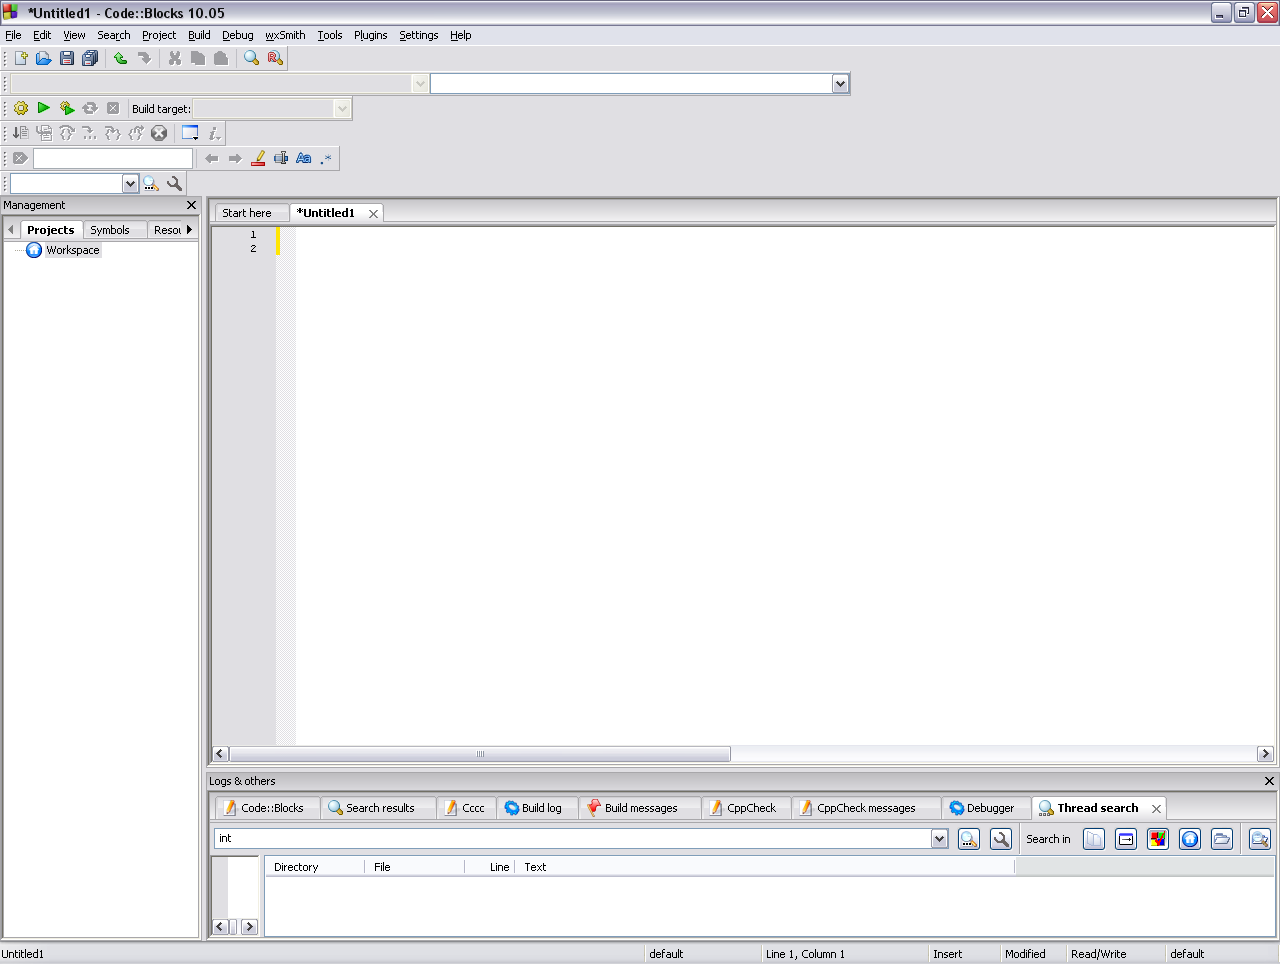
\includegraphics[scale=0.26]{images/cb_main}
\end{center}
\end{frame}

\begin{frame}{Елементи на главниот прозорец}
\begin{itemize}
  \item Лента со менија
    \begin{itemize}
      \item лентата со менија се наоѓа во најгорниот дел на прозорецот, веднаш под неговиот насловот 
      \item Во неа се наоѓаат менијата File, Edit, View, Search, Project, Build,
      Debug, wxSmith, Tools, Plugins, Settings, Help
    \end{itemize}
    \item Лента со алатки
    \begin{itemize}
      \item лентите со алатки (копчиња за стартување на најчесто користените
      команди на околината) се наоѓаат непосредно под лентата со паѓачки менија
    \end{itemize}
    \item Работна површина
    \begin{itemize}
      \item Потпрозорец за уредувачот на текст
      \item Прозорец за соопштенија.
      \item Прозорец за организација на работата на програмата
    \end{itemize}   
\end{itemize}
\end{frame}

\begin{frame}{Програмирање во C со Code::Blocks}{Креирање проект}
\begin{enumerate}
  \item Стартувајте CodeBlocks
  \item File -> New -> Project -> Empty Project -> Go 
\end{enumerate}
\begin{center}
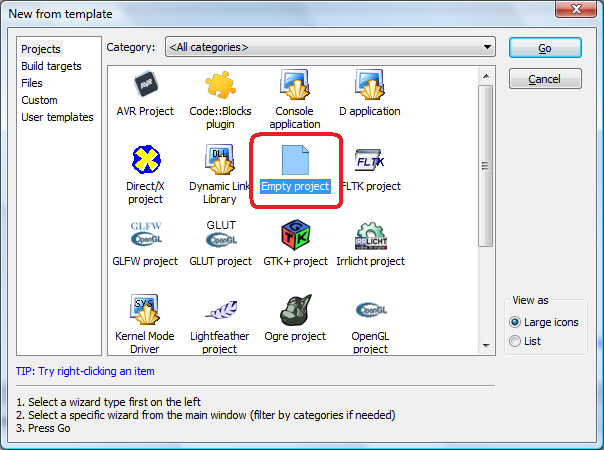
\includegraphics[scale=0.3]{images/cb_new}
\end{center}
\end{frame}

\begin{frame}{Програмирање во C со Code::Blocks}{Креирање проект}
\begin{enumerate}
\setcounter{enumi}{2}
  \item Одберете  GNU GCC Compiler
  \item Изберете ги следните 2 опции ако сакате да креирате “debug” и “release”
  configuration
\end{enumerate}
\begin{center}
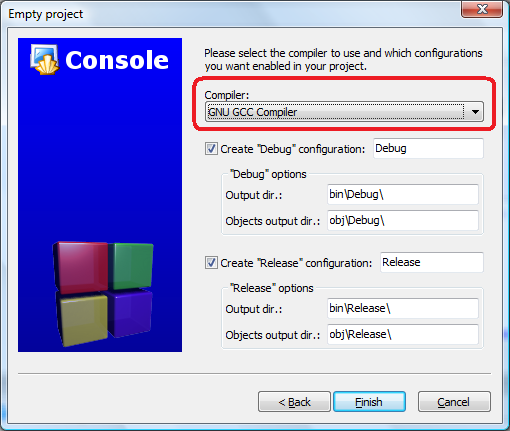
\includegraphics[scale=0.3]{images/cb_compiler}
\end{center}
\end{frame}

\begin{frame}{Додавање на изворна датотека}
\begin{enumerate}
\setcounter{enumi}{4}
  \item Додадете изворна датотека во проектот: File -> New -> File -> C/C++
  Source
  \item Одберете C како програмски јазик 
  \item Внесете го името на датотеката со полната патека и не заборавајте да го
  вклучите  "Add file to active project" 
\end{enumerate}
\begin{center}
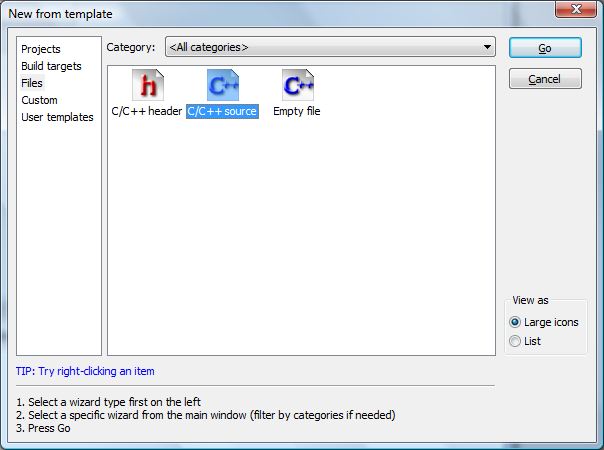
\includegraphics[scale=0.25]{images/cb_source}
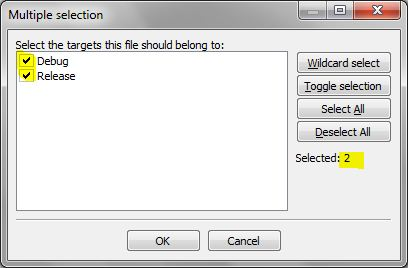
\includegraphics[scale=0.4]{images/cb_include}
\end{center}
\end{frame}

\begin{frame}{Програмирање}
\begin{itemize}
  \item За секој проект може да се постават следните опции "Project  Build Options..
Compiler Flags"
  \item За изградба на проектот (build) притиснете Ctrl + F9 
  \item За извршување на проектот притиснете Ctrl + F10
\end{itemize}
\begin{center}
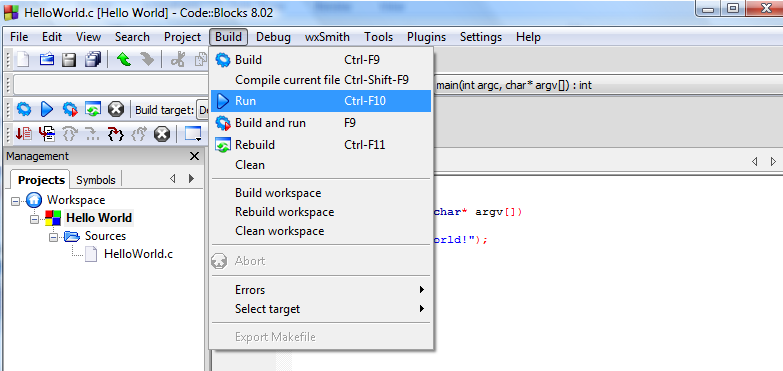
\includegraphics[scale=0.25]{images/cb_run}
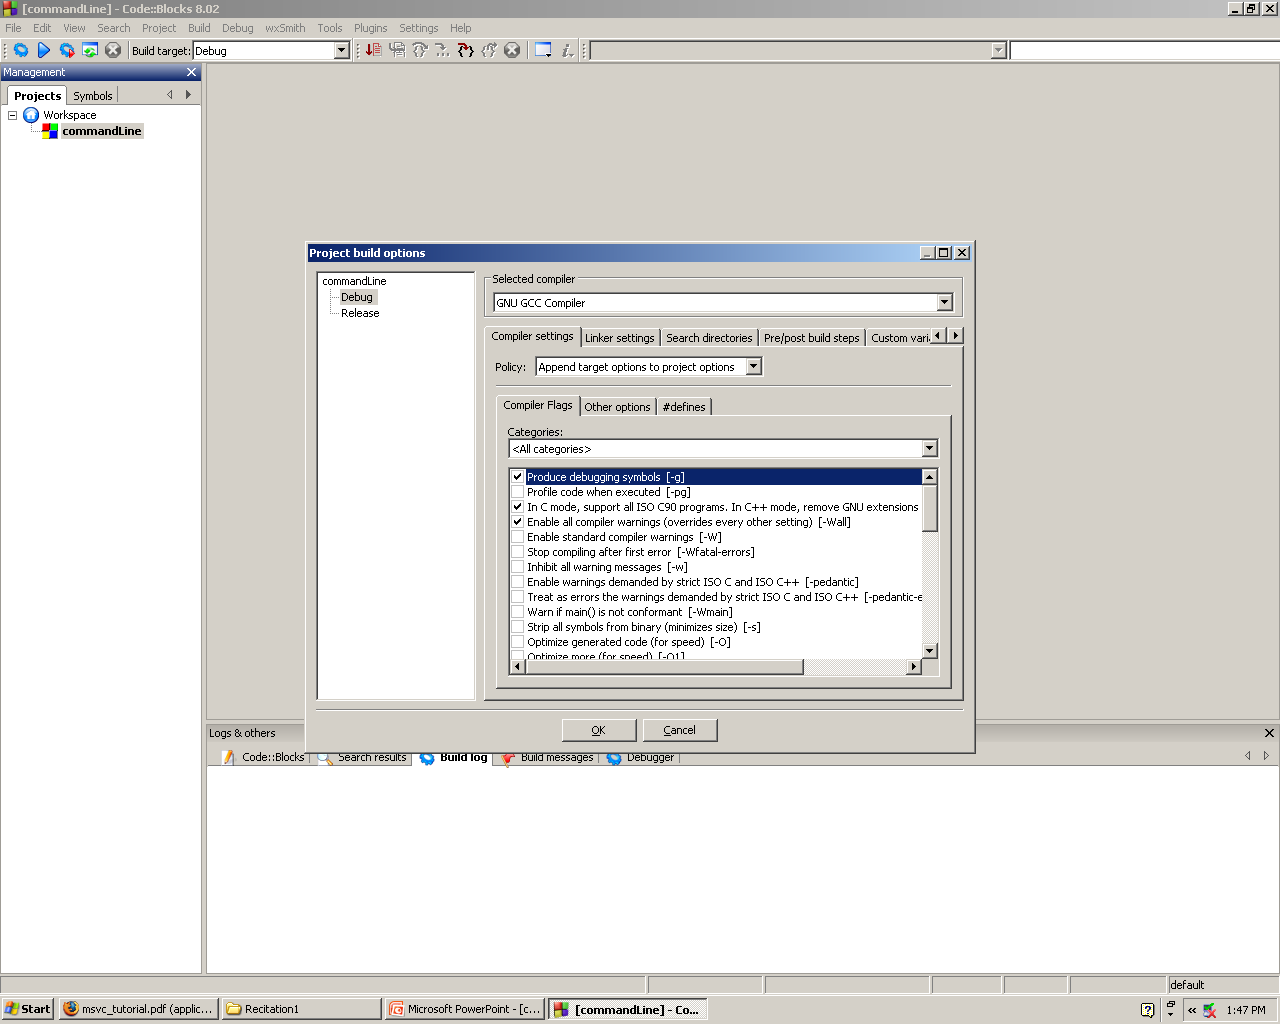
\includegraphics[scale=0.1]{images/cb_flags}
\end{center}
\end{frame}

\begin{frame}{Задачи за дома}
\begin{itemize}
  \item Во продолжение се наведени неколку задачи кои би требало да се обидете
  да ги изработите дома
  \item Со нивна изработка ќе бидете подготвени за успешна работа на
  претстојните лабораториски вежби
\end{itemize}
\end{frame}

\begin{frame}[fragile]{Задача 1}
Обидете се да креирате нов проект со една .с датотека и во неа внесете го
текстот на следнава програма:
\begin{lstlisting}
#include <stdio.h>

int main() {
    printf("Zdravo, kako si?\n");
    return 0;
}
\end{lstlisting}

\end{frame}

\begin{frame}{Задача 1}
\begin{itemize}
  \item Извршете ја програмата
\begin{itemize}
  \item Што добивате како резултат?
\end{itemize}
  \item Доколку сте направиле грешка при пишувањето на текстот поправете и
  извршете уште еднаш. 
  \item Направете намерно некоја грешка во текстот. Извршете повторно!
\begin{itemize}
  \item Што се случува сега?
\end{itemize}
\end{itemize}
\end{frame}

\begin{frame}[fragile]{Задача 2}
\definecolor{light-gray}{gray}{0.90}
Во текстот на програмата додадете до означениот ред:
\begin{lstlisting}[escapechar=!]
#include <stdio.h>
int main() {
    printf("Zdravo, kako si?\n");
    !\colorbox{light-gray}{printf("Neshto ne ti se pravi muabet?\n");}!
    return 0;
}
\end{lstlisting}
Кој е резултатот од извршувањето сега?
\end{frame}















